\section{Related Work}
The goal of this project was to create a new kickable and flickable interface for outdoors. For this, we first did some research about interactive systems that were designed for public spaces and interfaces that focused on feet interaction. Here, we present some interesting systems that inspired us during the creative phase of our work.
 
\subsection{Light bodies}
Seitinger, S. et al. \cite{seitinger} created the 'Light bodies': mobile and portable, hand-held lights that respond to audio and vibration input. Street lighting has changed over time and with it its relation to individuals. In the middle ages, each person used its own lantern. Then, in the beginning of 18th century, cities like Paris started to illuminate their streets at night; personal lanterns were not longer required. 'Light bodies' is an attempt to bring back the lost connection between lanterns and people and a medium to investigate the relationships between (urban) spaces, light and responsive, hand-held lights.'Light bodies' enabled people to directly and indirectly influence their personal lightscape.

In another related project, Seitinger, S. et al. \cite{seitinger-2} designed and implemented the 'Urban pixels': physically instantiated pixels that enable flexible, reconfigurable, unbounded, low-resolution, and responsive urban displays (see Figure~\ref{fig:urban-pixels}). 'Urban Pixels' are nodes in a wireless network of physical pixels for urban spaces. Each pixel unit includes a microcontroller, RF transceiver, LED module (ten bright, white LEDs), rechargeable Li-Ion battery pack, IR sensor and renewable energy source such as photo-voltaic cells. Users can interact with the 'urban pixels' by placing them spontaneously, by triggering sensors or by sending messages from their mobile devices. 

\begin{figure}[h!]
	\centering
	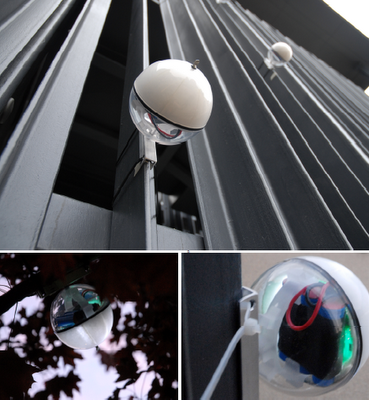
\includegraphics[width=0.2\textwidth, clip=true, keepaspectratio=true]{./pic/urban-pixels.png}
	\caption{Urban-pixels}
	\label{fig:urban-pixels}
\end{figure}

With this design, Seitinger, S. et al. \cite{seitinger-2} wants to present an opposite alternative to the majority of displays that are inflexible, flat, bounded, high-resolution and unresponsive. 


\subsection{Urban Cursor}

\begin{figure}[h!]
	\centering
	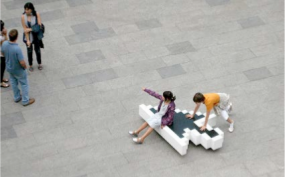
\includegraphics[width=0.5\textwidth, clip=true, keepaspectratio=true]{./pic/urban_cursor.png}
	\caption{Urban Cursor}
	\label{fig:urban_cursor}
\end{figure}

Another urban hci - project we recognized was the Urban Cursor.\newline 
Here, a team created a furniture, designed like a cursor. Approximately, its size is about two to three square metres. The whole thing is easy moveable, because of its wheels. The feature of the cursor is the GPS - tracking system. So the team could determine how the passers - by moved the furniture through the urban space.\newline
The cursor has a very large size because merely people should use it together, so that the project has a social aspect to.
[{\url{http://www.urbancursor.com}}] [09.09.2013] 

\subsection{Pixels Light Installation}

\begin{figure}[h!]
	\centering
	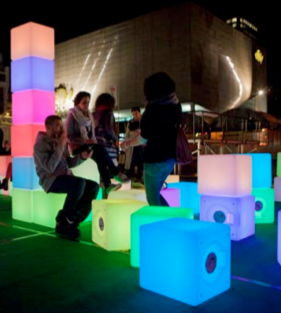
\includegraphics[width=0.5\textwidth, clip=true, keepaspectratio=true]{./pic/pixels_light_installation.png}
	\caption{Pixels Light Installation}
	\label{fig:pixels_light_installation}
\end{figure}
Here the designers built merely cube - devices. \newline
The idea was to built an installation similar to lego \texttrademark where a user can put those devices together or stack them to built different constructed forms. \newline
The cubes are color and intensity changing by rotation. Beyond that, each of the devices is direct and wirelessly connected to the others. So the environment is not driven by a server - client - system.\newline
By using the Arduino technology, those devices are using RF - and IF - sensors, so that they can recognize each other. So when they got kinetic input they will change their colour. With the connection the installation recognizes when some devices are put together, then the construct can be lighten up just in one colour. (All cubes are changing to that one colour.)\newline
 Furthermore the cubes are waterproof, so they can be used in the outside.\newline
\newline
[{\url{http://www.lightpublic.com/lighting-articles/get-pixelated-with-the-pixels-light-installation}}] [09.09.2013] \newline

\subsection{Liquid bricks}

\begin{figure}[h!]
	\centering
	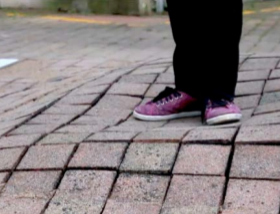
\includegraphics[width=0.5\textwidth, clip=true, keepaspectratio=true]{./pic/liquid_bricks.png}
	\caption{Liquid Bricks}
	\label{fig:liquid_bricks}
\end{figure}
 
This was a small urban project about a water - filled pouch. \newline
The idea was to built any furniture which can be used to make a fun for the passers - by. With this the team designed a texture seeming like the street's bricks. After that, they put the pouch to the ground - level of the street / square. So when a person was walking over it, it seemed like walking over a inconsistent place.\newline
\newline
[{\url{http://www.thisiscolossal.com/2011/06/liquid-bricks}}]\newline

\subsection{21 swings}

\begin{figure}[h!]
	\centering
	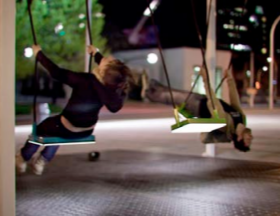
\includegraphics[width=0.5\textwidth, clip=true, keepaspectratio=true]{./pic/21_swings.png}
	\caption{21 Swings}
	\label{fig:21_swings}
\end{figure}

In Montreal a gigantic wings installation was created along a street.\newline
By swinging on a swing a music note is played. So when just one lonely passer - by is swinging, the system doesn't makes that fun. But when merely users are in action with the swings a hazard harmonic is in creation. \newline
Here the designers used the diatonic music system. This is the system which is known from playing harmonica: When the user is blowing in one specific hole, a tone will sound. When the user is suck in the same hole, the next tone in the musical scale will sound. Here in this project, each swing just gives one tone. It doesn't matter if the swing is swinging back- or forwards. The clue on this pattern is, that there cannot be any false note which doesn't match to the others.\newline
\newline
[{\url{http://www.fastcodedesign.com/1672192/watch-a-musical-swingset-forms-a-21-piece-orchestra}}]                
